%%%%% Document Setup %%%%%%%%

% \documentclass[12pt, onecolumn]{revtex4-2}    % Font size (12pt) and column number (one or two).

\documentclass[12pt, onecolumn]{article}


\usepackage{times}                          % Times New Roman font type
\usepackage{lipsum}
\usepackage{enumitem}

\usepackage{caption}
\usepackage{subcaption}

\usepackage[a4paper, left=2.5cm, right=2.5cm,
 top=2.5cm, bottom=2.5cm]{geometry}       % Defines paper size and margin length

\usepackage[normalem]{ulem}

\usepackage[sorting=none]{biblatex}
\addbibresource{references.bib}

\renewcommand{\baselinestretch}{1.15}     % Defines the line spacing

\usepackage[font=small, labelfont=bf]{caption}                      % Defines caption font size and caption title bolded

\usepackage{float}

\usepackage{graphics, graphicx, epsfig, ulem}	% Makes sure all graphics works

\usepackage{amsmath} 						% Adds mathematical features for equations
\usepackage{amssymb}

\usepackage{etoolbox}                       % Customise date to preferred format
\makeatletter
\patchcmd{\frontmatter@RRAP@format}{(}{}{}{}
\patchcmd{\frontmatter@RRAP@format}{)}{}{}{}
% \renewcommand\Dated@name{}
\makeatother

\usepackage{fancyhdr}

\pagestyle{fancy}                           % Insert header
\renewcommand{\headrulewidth}{0pt}
\lhead{\small Exploring Galaxy Morphology with Unsupervised Machine Learning}
\rhead{\small Samuel Howie}

\def\thesection{\arabic{section}}

\def\bibsection{\section*{References}}        % Position reference section correctly



\title{Exploring Galaxy Morphology with Unsupervised Machine Learning} 

\author{Samuel Howie}


\date{Supervisors: Prof C.M. Baugh, Dr T.Y. Cheng\\ \vspace{5mm} Level 4 Project, MSci Natural Sciences \\Department of Physics, Durham University \\ \vspace{5mm} Submitted: \today{}}

% \affiliation{\normalfont Level 4 Project, MSci Natural Sciences \\ Supervisors: Prof C.M. Baugh Dr T.Y. Cheng\\ Department of Physics, Durham University}



%%%%% Document %%%%%
\begin{document}                     

    
\maketitle


% \maketitle
%\thispagestyle{plain} % produces page number for front page


\begin{abstract}              

Abstract abstract abstract abstract abstract abstract abstract abstract abstract abstract abstract abstract abstract abstract abstract abstract abstract abstract abstract abstract abstract abstract abstract abstract abstract abstract abstract abstract abstract abstract abstract abstract abstract abstract abstract abstract abstract abstract abstract abstract abstract abstract abstract abstract abstract abstract abstract abstract abstract abstract abstract abstract abstract abstract 

\end{abstract}

\newpage

\tableofcontents

% \let\toc@pre\relax
% \let\toc@post\relax

\newpage

\section{Introduction}

    % \subsection{Motivation \& Aims}

    \subsection{Classification of Galaxy Morphology}
        % \begin{enumerate}
        %     \item Why is Galaxy Morphology Important (look at how galaxies evolve with redshift, we can look at multiple redshifts and compare (arxiv.org/abs/2306.17225)
        %     \item What are the current classification methods in place (eg. Hubble)
        %     \item Why are these bad
        %     \item What have other people done to try to fix it (eg. extending visual classification, other non visual methods)
        %     \item Why are those methods also bad (visual classification doesn't work on high redshift galaxies)
        % \end{enumerate}

        Galaxy morphology plays a pivotal role in understanding the physical processes within galaxies and provides a record of their evolutionary history \cite{high_redshift_UL}. For example, bulge-dominated galaxies, such as elliptical galaxies, are generally red in colour, which indicates the stars have stopped forming within the galaxies \cite{elliptical_red_low_sfr}, as well as massive \cite{elliptical_massive} and rich in merger history \cite{bulge_rich_merger_history} where the strength of the bulge is correlated with the number of mergers \cite{bulge_strength_no_mergers}. In contrast, disk-like galaxies, such as spiral galaxies, tend to be bluer in colour \cite{blue_spiral}, less massive \cite{spiral_low_mass} and unlikely to have had any significant mergers \cite{disk_low_mergers}.
        
        The Hubble sequence \cite{original_hubble_sequence} is the most popular galaxy classification system and groups galaxies, based on their appearance, into elliptical and spiral galaxies, with the addition of other fine types such as lenticular galaxies and barred spiral galaxies from other following works \cite{lenticulars} \cite{deVaucouleurs_system}.
        
        At $z \sim 0$, research indicates that approximately 72\% of galaxies are spiral galaxies, 13\% are lenticular, 3\% are elliptical and only 10\% fall into the category of irregular galaxies \cite{hubble_sequence_6_Gyr_ago}. Irregular galaxies are galaxies which don't fit into any specific category. This suggests that the Hubble sequence could accurately classify the majority of galaxies that Hubble had access to at the time. 

        However, with modern observational techniques, such as the Hubble Space Telescope \cite{hst} and ground-based CCD cameras such as the Sloan Digital Sky Survey \cite{sdss}, among others, an increasing number of peculiar galaxies have been observed, particularly at higher redshifts. Research suggests that at $z \sim 0.5$, 52\% of galaxies are classified as peculiar \cite{hubble_sequence_6_Gyr_ago} indicating that the Hubble sequence becomes less effective at higher redshift.
        
        % However, with the launch of the Hubble Space Telescope in 2000, there has been increasing number of peculiar galaxies observed at higher redshift. Research suggests that 52\% of galaxies are classified as peculiar at redshift $z \sim 0.5$ \cite{hubble_sequence_6_Gyr_ago} indicating that the Hubble sequence becomes less effective at higher redshift.

        ************************

        While some of the limitations of the Hubble sequence have been addressed by breaking down the original Hubble classes, such as de Vaucouleurs, who further broke down spiral galaxies based on the presence of inter and outer ring structures \cite{deVaucouleurs_system}, there is an inherent bias originating from the Hubble sequence present in these visual classification schemes.    

        ************************

        

    \subsection{Machine Learning Application to Galaxy Morphology}
        % \begin{enumerate}
        %     \item Why ML can be better (eg. efficiency, accuracy
        %     \item How was supervised learning been used for galaxy morphology (Huertas-Companyetal. (2015)createdaCANDELScataloguewhichreliedon8000expert classificationsofgalaxies in GOODS-SouthtotraintheConvNet toclassifytheremainderof theCANDELSintofivevisual-likemorphologies:disk,spheroid, peculiar/irregular,point source/compactandunclassifiable)
        %     \item What are the problems with supervised learning (training set might miss certain types of galaxies, human bias with supervised)
        %     \item Why would you therefore go with unsupervised learning
        %     \item How has unsupervised learning been used for galaxy morphology
        %     \item What are the issues with unsupervised learning (number of extracted features, how many different types of galaxies are there (the things I am trying to figure out)
        % \end{enumerate}


        % The James Webb Space Telescope is capable of observing galaxies at redshift  $z\gtrsim 15 $ \cite{JWSP_largest_redshift} resulting in a huge number of observable galaxies. The sheer number of galaxies is far too high for any human visual classification system to process. The use of machine learning to assist with galaxy classification therefore becomes essential.

        Modern surveys such as the Sloan Digital Sky Survey (SDSS) ($\sim$ 50 million galaxies) \cite{sdss} and the Dark Energy Survey ($\sim$ 300 million galaxies) \cite{des} are capable of observing such large numbers of galaxies that manual classification is far too difficult. The use of machine learning to assist with galaxy categorisation therefore becomes essential.

        Early applications of machine learning to morphological classifications, such as Dieleman \cite{first_ml_galaxy_application} (the first application of convolutional neural networks) made use of unsupervised learning. This requires the model to train on a pre-labelled dataset. The largest example of this is the Galaxy Zoo \cite{gal_zoo_original}. A huge group of volunteers ($\sim$ 100,000) manually classified $\sim$ 900,000 galaxy images from the SDSS \cite{gal_zoo_no_galaxies}. These classified galaxies can then be used to train unsupervised learning models which can then be applied to catagorise other SDSS galaxy images.

        Supervised learning can make very accurate predictions, for example, Dieleman's model can reproduce Galaxy Zoo classifications with $>$ 99\% accuracy \cite{first_ml_galaxy_application}. However, there is an inherent bias. Because there is a *********************************************




        
        
        Because the specific categories of galaxies are already decided,  the model can't ident presence of any other categories that are not considered in the training set 
        
        
        doesn't allow for the presence of any other categories that are not considered in the training set.
        
        For example, Dieleman  the first application of convolutional neural networks to morphological classfification, 
        
        The first applications of machine learning to galaxy morphology by Dieleman \cite{}

        For example, Dieleman 
        
        For example, categorising galaxies into early and late type with an accuraxy of 96.4%

        
        

        % For instance, supervised learning has been applied to the classification of a sample of \break 316 013 galaxies from the Sloan Digital Sky Survery \cite{sloan_digital_sky_survey} into early and late type galaxies with an accuracy of 96.4\% \cite{supervised_ml_morphology}. Although supervised learning is very useful to classify a huge number of galaxies into a predetermined classification system, there is an inherent bias. The fact that the specific categories of galaxies are already determined doesn't allow for the presence of any other categories that are not considered in the training set.

        % Utilising unsupervised learning requires the machine to identify its own patterns and extract the features it thinks are most important with no previous knowledge of any other galaxy classification systems. This removes the bias present in supervised learning models. Additionally, unsupervised learning isn't limited to a predefined number of possible categories, as is the case with supervised learning.
        
        % Computers look at images on a pixel-by-pixel level facilitating the analysis of images at a level of detail far beyond human capabilities thereby picking out intricate patterns and details humans can't. This can potentially allow for the identification of physical galaxy properties which typically can't be obtained by visual inspection.

        

        
    
        

    \subsection{Project Aims}
        % \begin{enumerate}
        %     \item What am I proposing (see what the extracted features are and find the most optimal number
        %     \item Overview of each section (second 2 I'll talk about the dataset etc)
        % \end{enumerate}

        This project aims to revisit the Hubble sequence with modern data to form an unbiased morphology classification system.
        
        I have developed an autoencoder neural network to make use of unsupervised machine learning. I use this to extract features from individual galaxy images, subsequently utilizing clustering algorithms on these features to categorise galaxies with similar characteristics. The extracted features are also compared to structural and physical galaxy properties, obtained from the EAGLE database \cite{eagle_catalogue_public_release}, which can be used to analyse the different categories of galaxies to see how they have been grouped.

        Additionally, this project aims to find the optimal number of extracted features using an autoencoder for effective galaxy categorisation. This involves extracting a sufficient number of features to maintain model accuracy while also ensuring that they remain astronomically and scientifically meaningful (see section \ref{no_extracted_features}).

        In Section \ref{Dataset}, I will describe the dataset used for the project, as well as the pre-processing procedure for data preparation. In Section \ref{Methodology}, I will describe my unsupervised machine learning approaches composed of feature extraction using autoencoder and categorisation with clustering algorithms. In Section \ref{Results}, I will explain what the extracted features tell us about the galaxies and how they have been categorised. 

        \vspace{5mm}
        ***********************
        
        I will give a summary in Section \ref{Conclusions} and in Section \ref{Future Work} talk about how the project could be extended in the future.

    
    
    % \begin{enumerate}
    %     \item Why is Galaxy Morphology Important
    %     \item What are the current classification methods in place (eg. Hubble)
    %     \item Why are these bad (visual classification)
    %     \item What have other people done to try to fix it (eg. extending visual classification, other non visual methods)
    %     \item Why are those methods also bad
    %     \item What am I proposing
    %     \item Why unsupervised and not supervised (training set might miss certain types of galaxies, human bias with supervised)
    %     \item Why is that better (remove bias, visual scheme missing something, increase efficiency, we now have so many (300 million) that we can't do it by manually, need a computer to do it)
    %     \item We can investigate the point where the machine picks more detail than the human eye 
    %     \item Applications to other simulations and real images (may have to change model eg. different number of extracted features)
    %     \item Other applications of ML in atro
    % \end{enumerate}




    % In 1926, Edwin Hubble devised the Hubble Sequence, a way to categorise galaxies by their appearance \cite{hubble_sequence}. This involved categorising them into three main groups, elliptical galaxies, lenticular galaxies and spiral galaxies. 
    
    % % Elliptical galaxies are numbered from E0 to E7, where E0 is essentially round and E7 is very elliptical, and spiral galaxies were assigned letters Sa to Sc which correspond to how tight the spiral arms are. Lenticular galaxies are labelled S0. Like spiral galaxies, lenticular galaxies are disk-like structures but have no spiral structure. Spiral galaxies were also grouped into an additional two groups, normal spiral galaxies and barred spiral galaxies (given the symbol SBa-SBc), where the galaxy's centre is shaped like a bar, rather than the round centre of a normal spiral galaxy \cite{hubble_sequence}.
    
    % \vspace{5mm} 
    % \noindent *** Diagram of Hubble Sequence
    % \vspace{5mm}
    
    % This way of categorising galaxies worked well for the local galaxies (galaxies within the Milky Way which has a diameter of around 10 million light-years) \cite{local_galaxy} that Hubble had to work with. In the local universe, it has been found that around 72\% of galaxies are spiral and only 10\% are peculiar \cite{hubble_sequence_6_Gyr_ago}. Peculiar galaxies are galaxies which don't fit into any specific category \cite{peculiar_galaxies} so given in the local universe, only 10\% of galaxies are categorized as peculiar, the Hubble sequence works well here.
    
    % However, we can now look much further into space and time and see many more galaxies and at different time periods. This resulted in an increasing number of galaxies being categorized as peculiar. For distant galaxies 6 billion light-years away, only 31\% are spiral galaxies and 52\% are peculiar \cite{hubble_sequence_6_Gyr_ago} showing that the Hubble sequence isn't categorising the majority of galaxies.
    
    % Talk about De Vancoulers extension of the Hubble sequence \cite{deVaucouleurs_system}. How many galaxies are now peculiar? Talk about spectral categorising and how that is better.
    
    % All of these categorization methods are, to an extent, extensions of previous methods which leads to bias as we decide what constitutes a particular category. If we made use of machine learning, we would remove any sort of human bias coming from any previous categorising methods. The machine learning model would look at a set of galaxies, pick out its own features, which could be very different to those picked out by the human eye, and categorise them accordingly. Computers can also see much more detail compared to the human eye, and this could result in the model picking out information that humans wouldn't be able to just by looking at an image of a galaxy and this information could relate to very useful galaxy properties.

\newpage

\section{Dataset}
\label{Dataset}

    \subsection{EAGLE Simulation}
    
        % \begin{enumerate}
        %     \item[-] What is the EAGLE Simulation (physics behind it eg. how the galaxies are formed, parameters that go into this eg. formation properties, supernova feedback and agm feedback)
        %     \item[-] What specific simulation are we working with (eg. boxsize and redshift)
        %     \item[-] Disadvantages of EAGLE (eg. massive galaxies not representative and why they aren't)
        % \end{enumerate}
        
        % Distrubution of galaxies eg. how many types of elliptical, spiral etc, how many images resized
        
        % Pro and cons of using simulation data eg. massive galaxies are not that representative of real galaxies


        The EAGLE project \cite{eagle_schaye} is a suite of hydrodynamical cosmological simulations. These simulations follow the formation of galaxies and supermassive black holes within cosmological volumes of a highly representative $\Lambda$ CDM universe. \cite{eagle_schaye}.

        The simulations are created using a modified version of the GADGET code (n-body simulation using smoothed particle hydrodynamics \cite{gadget_code}). Enhancements include a modified hydrodynamics solver, time-step limiter and most importantly the subgrid physics \cite{eagle_catalogue_public_release}.

        % Summarise the following enhancements to the subgrid physics from \cite{eagle_schaye} (one or two sentences each, or pick out the most important ones and give a paragraph each?):
        % 
        % \begin{enumerate}[itemsep=0mm]
        %     \item[-] Radiative cooling
        %     \item[-] Star formation 
        %     \item[-] Stellar mass loss
        %     \item[-] Energy feedback from star formation
        %     \item[-] Dependence on local gas properties
        %     \item[-] Black holes and feedback from AGN
        % \end{enumerate}

        Star formation rate (SFR) is taken to depend on density rather than pressure. This offers two main advantages, firstly, no tuning is required for the Kennicutt-Schmidt star formation law \cite{kennicutt–schmidt_star_formation_law} given we can use observations of the gas and star formation rate surface densities \cite{eagle_schaye}. Additionally, no recalibration is required under a change of state, as would be required with a pressure-dependent star formation rate \cite{eagle_schaye}.

        Mass loss is implemented based on the Wiersma's method \cite{mass_loss}. At each time step, the stellar masses reaching the end end of their main-sequence phase are computed. The mass loss is distributed among neighbouring smoothed particle hydrodynamic (SPH) particles with adjustments to conserve momentum and energy. During these calculations, unlike the Wiersma's method, a fixed initial particle mass is used to avoid biases during these calculations \cite{eagle_schaye}.

        Black holes can form in a variety of ways. Since the simulation cannot resolve very small scales such as the collapse of metal-free dwarf galaxies or the remnants of massive, metal-free stars, the Springel's method \cite{bh_seeds} is implemented. This places a black hole seed at the centre of every halo with a total mass $> 10^{10} M_{\odot} h^{-1}$. At every time step, the location of the black hole is moved to the position of the particle with the lowest gravitational potential among its neighbouring particles. \cite{eagle_schaye}.
        
        Stellar populations inject energy into the interstellar medium (ISM) through supernovae, stellar winds and radiation. This is known as stellar feedback and is implemented for each star individually based on the thermal feedback scheme described by Dalla Vecchia \& Schaye \cite{stellar_feedback}. A temperature change is set representing the increase in temperature for stochastically sampled gas particle neighbours. The value of this temperature change strikes a balance, being high enough to remove significant numerical losses and low enough to prevent the probability of heating neighbouring particles from becoming too small resulting in inadequate sampling \cite{trayford}.

        \vspace{5mm}
        ***********************
        
        AGN Feedback
        
        % Only a single mode of AGN (active galactic nucleus) feedback is implemented to reduce the number of feedback channels to the minimum required to be consistent with observations. Energy is injected thermally at the location of the black hole at a rate that is proportional to the gas accretion rate \cite{eagle_schaye}. This implementation is similar to quasar-mode feedback where the black hole is efficiently accreting in the form of hot, nuclear wind \cite{eagle_schaye}. 

        
        

        

        
        
    
    \subsection{Mock Galaxy Images}
        % \begin{enumerate}
        %     \item Introduction about Trayford's work - what have they done to make EAGLE images look like observed mages (SDSS)
        %     \item What kind of images are we working with (eg. resolution, 3-bands)
        %     \item How many galaxies in the samples, what are their properties (eg. distribution of galaxies and their physical properties, any biases?)
        % \end{enumerate}

        The EAGLE database provides images from various simulations of differing box sizes ranging from 25 to 100 comoving Mpc (cMpc) \cite{eagle_catalogue_public_release}) at varying snapshots for redshift $z=0$ to $z-20$ \cite{eagle_catalogue_public_release}. For this project, I use images from Trayford et al. \cite{trayford} which sample the RefL0100N1504 simulation which has a box size of 100 cMpc at redshift $z=0.1$.

        With the largest volume of the EAGLE simulations, i.e. 100 cMpc, only galaxies with stellar mass $M_{*} > 10^{10} M_{\odot}$ have been sampled, resulting in a sample of 3624 galaxies.
        
        The images are made up of mock fluxes at a distance of 20Mpc corresponding to the SDSS (Sloan Digital Sky Survey) $u$, $g$ and $r$ band filters \cite{how_images_taken}, centred around wavelengths 3500\AA, 4800\AA\ and 6200\AA\ respectively. This gives us 3-band images and each has a resolution of 256$\times$256 pixels.

        To make these images more representative of observed galaxy images, the effects of dust have been taken into account utilizing the SKIRT code \cite{trayford}.

        Gravitational softening (angular resolution) ******

        how many images

        \vspace{5mm}
        ************************************
        
        Explain what the SKIRT code does

        ************************************
    
        
        \subsection{Data Preparation}
        
        \subsubsection{Image Normalisation}
        
            % \begin{enumerate}
            %     \item[-] Why do we have to normalise the images (eg. to ensure we are not taking into account colour)
            %     \item[-] Why don't we want to take into account colour (eg. colour  usually a good indicator (why?),  dust makes a galaxy appear more red, and we do get some red spirals and blue ellipticals) 
            % \end{enumerate}

            The colour of a galaxy provides useful information. For example, redder galaxies are typically much older and less massive than bluer galaxies, and the stars within have stopped forming. \cite{elliptical_red_low_sfr}.

            However, intervening dust can absorb and scatter light from stars. This effects blue light more due to the shorter wavelength. This means that galaxies with high amounts of dust appear redder. The colour of a galaxy can therefore be quite misleading.

            We therefore want to minimise the effect of colour within the model. To do this, the three bands have each been normalised between 0 and 1 (where 0 is dark and 1 is bright). This prevents specific bands from being much more prominent than others and minimises the effect of colour in the model.

            
    
        \subsubsection{Image Resizing}
        
            % \begin{enumerate}
            %     \item[-] Why do I have to resize some galaxies
            %     \item[-] How many galaxies do I have to resize
            %     \item[-] What do the galaxies look like after they have been resized
            %     \item[-] How am I resizing the images 
            % \end{enumerate}

            Although I am sampling galaxies with stellar mass $M_{*} > 10^{10} M_{\odot}$, there is still a large range of stellar masses within the sample ($\sim 10^{10} M_{\odot}$ to $\sim 5\times10^{11} M_{\odot}$). This results in a large range of sizes of galaxies, with the less massive galaxies typically appearing to be much smaller.

            The model therefore immediately starts grouping galaxies together based on their apparent size, rather than more meaningful galaxy properties, such as the Sersic index, among others, (see Sections \ref{structual_measurements} and \ref{physical_propeties}).

            To overcome this, I have developed an algorithm to identify these smaller galaxies by the width of their light intensity profile. I then crop to the centre of these images, doubling the apparent size of the galaxies. The remaining images have been scaled down to the same resolution as the cropped images. The galaxy images now have a resolution of 128$\times$128.


            

            % I have identified a specific subset of the galaxy images (********* number *********) that are significantly smaller than the rest. If left untouched, the model immediately picks these out as specific groups, rather than categorising the galaxies on more scientifically and astronomically meaningful properties. 

            % I have developed an algorithm to identify these galaxies. These smaller galaxies have a much narrower light intensity profile and I have chosen a cutoff 

            
            % We need to make sure we are categorising our galaxy images based on meaningful galaxy properties rather than arbitrary image properties.
            
            % Currently, the most obvious difference between any two images in this dataset is the size of the galaxies, or rather the apparent size of the galaxies. Our dataset is comprised of images of galaxies at different distances from the observer. This may lead the model to think that some galaxies are much smaller when in reality they are just further away from the observer. We therefore want our images to appear to be similar in size so the model categorises them based on more meaningful visual properties.
            
            % The best way that I have found to do this is to make use of the 2D intensity profile of the galaxies. For the x-axis, this is obtained by averaging out the pixel values across the entire y-axis for each pixel in the x-axis. We can take the same approach for the y-axis. I then divide these two intensity profiles by the mean pixel value for the entire image, giving the intensity profiles as a ratio of the mean intensity of the image. This stops the apparent magnitude of our galaxies affecting our resizing algorithm, another property which we would like our model to ignore. I then find the two points at which our intensity profile drops to half the maximum intensity (as a ratio to the mean intensity) and calculate this range. Essentially, if you were to plot this profile, I would be calculating the full width at half maximum for each image. This then tells us how much of each image is taken up by the galaxy itself rather than just empty space.
            
            % Ideally, I would crop all images based on this range so every image has a very similar apparent size. Unfortunately, this isn't possible because for the model to work, all images need to be the same size. This means we must either crop or upscale all images to the same resolution.
            
            % I have realised that there is a distinct group of images where the galaxy takes up a significantly smaller amount of the image than the others. These are therefore immediately picked out by our clustering algorithm (explained in section \ref{Clustering}) as two groups which is exactly what we are trying to avoid here. I will therefore use this resizing algorithm to enlarge these 'smaller' galaxies to increase their apparent size to a much comparable value to the others.
            
            % I therefore pick a cutoff point for the full width at half maximum which filters out these 'smaller' galaxies from the rest. I have chosen here to pick that cutoff range of 60 pixels meaning that the majority of the galaxy has to be located within the middle 60 pixels to be identified as a small image. I then crop these images to only take the central region, reducing the image size by half. For the remaining images, to ensure that they have the same dimensions as the cropped images, I scale these down. We pan across the whole image finding all 2x2 regions. We then find the average pixel value of all these regions and form a new image out of these averages, reducing the size of the image by half.
            
            
            % \begin{figure}[H]
            %     \centering
            %     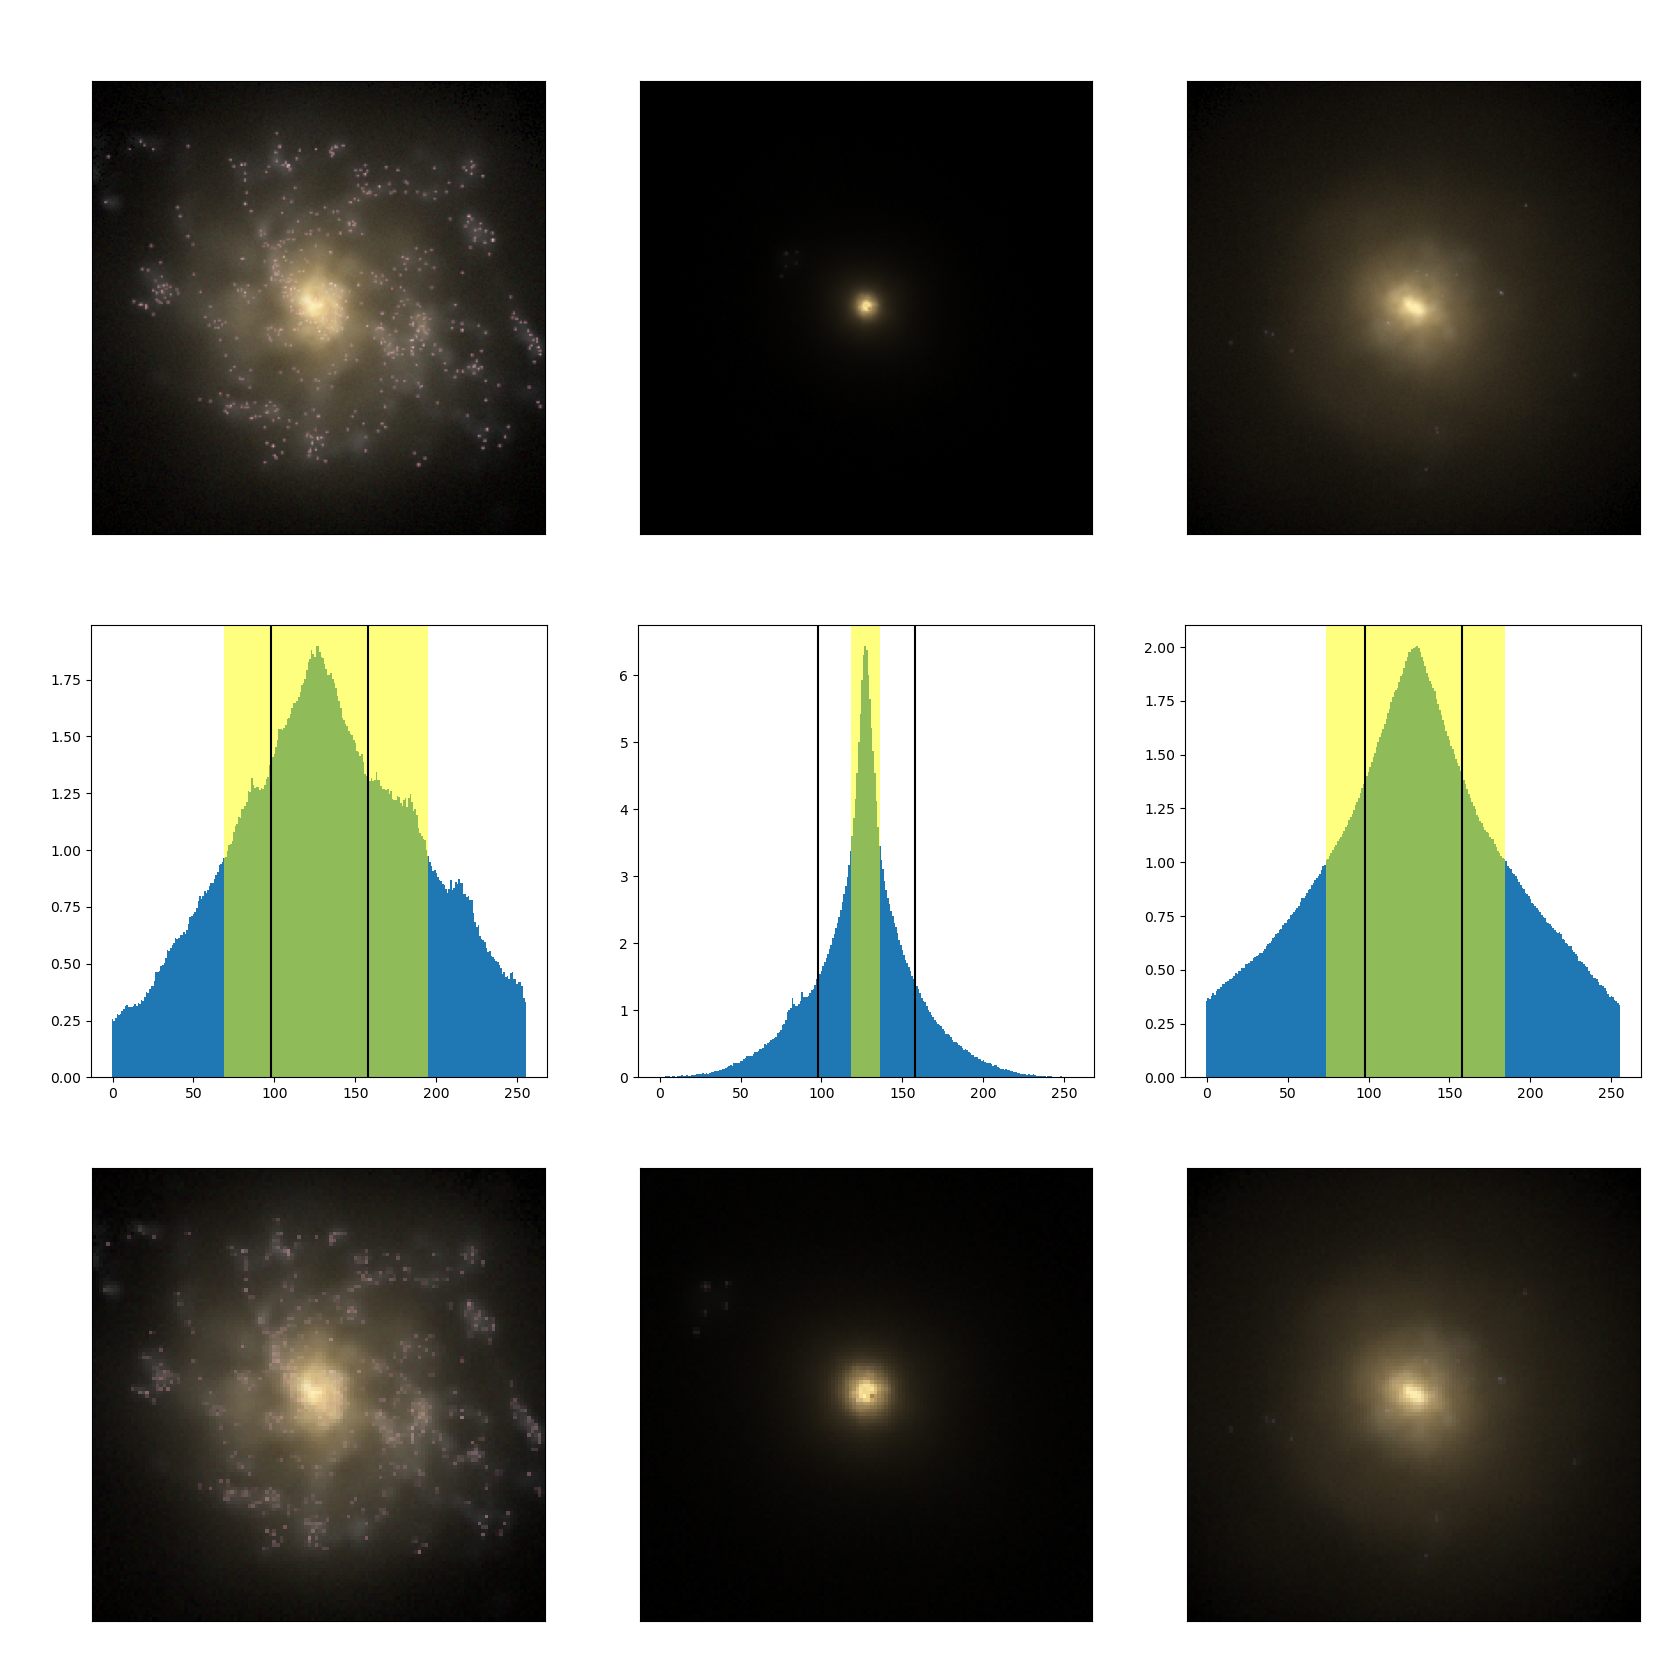
\includegraphics[width=0.75\textwidth]{Images/resize_image_demo.png}
            %     \caption{Representation of image resizing}
            %     \label{Image Resizing}
            % \end{figure}
            
            
            % In the top row of Figure \ref{Image Resizing} we can see three images, the centre of which shows one of these 'smaller' galaxies. In the middle row, we can see the intensity profile as a ratio of average intensity, along with the full width at half maximum, shown in yellow, and our chosen cutoff range shown by the black vertical lines for each of the three images. We can see that only the central galaxy image is identified as a small image as it is the only one with a full width at half maximum within the cutoff range. The bottom row shows the images after they have gone through the resizing algorithm. As expected, we have cropped into the central image and have scaled down the outer images, retaining their apparent size.
            
            % As shown in the bottom row, cropping the central image and scaling the other two down brings the apparent size of the central galaxy up to a value similar to the other two. It is still noticeably smaller and reducing the image size further would make the apparent size much more comparable but this would result in a large large loss of detail within the images being scaled down. I think reducing the image resolution by half strikes the best balance between retaining image detail and similar apparent sizes.

        \subsection{Summary}

            Quick summary of the images used for the project
    
    
    % \subsection{Overview of Machine Learning}
    % \label{Machine Learning}
    
    % Explain how machine learning and neural networks work (with maths). Start with supervised learning (given it is easier to understand) and then explain unsupervised learning and then explain autoencoders. Use the example of a computer reading handwritten numbers as it is an easy to understand analogy. This is more of an intro for people who don't have any experience with machine learning, I won't be talking about the specific model I am using for the project, that will explained in section \ref{Model}
    
    % \subsubsection{Supervised Learning}
    
    % ...
    
    % \subsubsection{Unsupervised Learning}
    
    % ...
    
    % \subsubsection{Autoencoders}
    
    % ...
    
    
\newpage

\section{Methodology}
\label{Methodology}

    % For this project, I have developed an autoencoder neural network to make use of unsupervised machine learning. I use this to extract features from each galaxy image which are then used to categorise and group similar galaxies. The extracted features are also compared to known galaxy properties for each image to see if the model is extracting meaningful information.
    

    Machine learning enables a computer to learn directly from data  \cite{what_is_ml}. Essentially, machine learning looks to mimic the human brain through the use of artificial neural networks \cite{first_neural_network}. 
    
    In this project, I use an unsupervised learning approach which requires the model to train on an unlabelled dataset. This kind of approach involves extracting representative features from data (i.e. galaxy images in our case) and identifying a pattern that can help grouping samples in the feature space.

    For feature extraction, I have developed an autoencoder. An autoencoder is essentially the combination of two models, an encoder and a decoder. The encoder takes the data, in our case, images of galaxies, and breaks each down into a one-dimensional latent representation. The decoder does the opposite, it builds back up from that one-dimensional representation to form a reconstruction of the original image. The middle layer of the autoencoder contains the latent representation (extracted features) of images. Each image can then be described by a set of latent features

    The performance of an autoencoder is assessed based on the similarity between the model's reconstructions and the original images. Accurate reconstructions imply that the model has extracted accurate representations of the original images.



    \vspace{10mm}
    *******************
    Diagram of Autoencoder
    *******************
    \vspace{10mm}


    
    
    
    \subsection{Feature Extraction}
    \label{Feature Extraction}

        As discussed in Section \ref{Dataset}, I am transforming 3-band, 128$\times$128 images (giving an image shape of 128$\times$128$\times$3) down to a one-dimensional latent representation of size 
        
        \vspace{5mm}
        *******************
        number of extracted features 
        *******************
        \vspace{5mm}
        
        . To do this, I will be using the layers shown in Figure \ref{autoencoder_layers} to gradually reduce the dimensionality from 128$\times$128$\times$3 down to 32. Gradual dimensionality reduction is very important as it allows the model to pick out more intricate patterns leading to more scientifically meaningful extracted features \cite{dnn_feature_extraction}.


        \begin{table}[H]
            \centering
            % \begin{tabular}{|p{0.2\linewidth} p{0.2\linewidth} p{0.1\linewidth} p{0.1\linewidth} p{0.1\linewidth} p{0.15\linewidth}|}

            \begin{tabular}{c c c c c}
                
                Layer Type & Output Shape & Stride Size & Activation Function  \\
    
                \hline\hline
                
                Convolutional & 128$\times$128$\times$64 & 2$\times$2 & ReLu \\
    
                Convolutional & 64$\times$64$\times$32 & 2$\times$2 & ReLu \\
    
                Convolutional & 32$\times$32$\times$16 & 2$\times$2 & ReLu \\
    
                Convolutional & 16$\times$16$\times$8 & 2$\times$2 & ReLu \\
    
                Convolutional & 8$\times$8$\times$4 & 2$\times$2 & ReLu \\
    
                Flatten & 256 & & \\

                Dense & 64 & & \\
                
                Dense & ******* & & \\
    
                \hline
    
                Dense & 64 & & \\
    
                Dense & 256 & & \\
    
                Reshape & 8$\times$8$\times$4 & & \\
    
                Transposed Convolutional & 16$\times$16$\times$4 & 2$\times$2 & ReLu \\
    
                Transposed Convolutional & 32$\times$32$\times$8 & 2$\times$2 & ReLu \\
    
                Transposed Convolutional & 64$\times$64$\times$16 & 2$\times$2 & ReLu \\
    
                Transposed Convolutional & 128$\times$128$\times$32 & 2$\times$2 & ReLu \\
    
                Transposed Convolutional & 128$\times$128$\times$3 & 1$\times$1 & Sigmoid \\


            \end{tabular}
            \caption{Description of each of the layers of the autoencoder. The top half is the encoder and the bottom half is the decoder. All convolution and transposed convolution layers have a kernel size of 3$\times$3}
            \label{autoencoder_layers}
        \end{table}


        
        
        % The middle layer of the autoencoder determines the dimensionality of the latent representation of the encoder. The dimensionality is just how many features we want to extract from each image. Each extracted feature, for each image, has a number associated to it. For example, if we have 1000 images and want to extract 10 features, for each of the 1000 images, we would have 10 different numbers.

        The middle layer of the autoencoder (output of the encoder) contains the latent representation (extracted features) of images. Each image can then be described by a set of latent features
        
        The values of the extracted features aren't necessarily associated to anything that humans can comprehensively recognise. The machine identifies its own patterns and extracts the features it considers are most important to reconstruct the input images with no with no previous knowledge of any other galaxy classification systems. In section \ref{Representation of the Machine Features} we discuss how some of these extracted features are correlated with galaxy properties.

        
        % The more extracted features we have, the more information we have about the images. This means we can make more accurate reconstructions of the galaxies if we feed the extracted features into the decoder of our model. However, if we try to extract too many features, they may become meaningless. The aim of this project is to categorise galaxies and to try to make the model pick out some galaxy properties, not to make the most accurate reconstructions of galaxies possible. This means we have to strike a balance between extracting enough features to make somewhat accurate reconstructions, but not too many so the features we do extract are meaningful. I have found that the best balance for the dataset used has been 32 features.

        The number of extracted features used in an autoencoder decides how much information can be encoded in each image. In Section \ref{no_extracted_features}, we discuss how more extracted features leads to better reconstructions of images. However, if too many features are extracted, they start to become less scientifically and astronomically meaningful.
        
        The aim of this project is to use these extracted features to categorise galaxies rather than produce the most accurate reconstruction of galaxy images. We therefore have to find an adequate number of features that can produce good reconstructions but remain astronomically and scientifically meaningful. The most optimal number I found for this work is 
        
        \vspace{5mm}
        ******************* number of extracted features *******************
        \vspace{5mm}
        
        features, as discussed in Section \ref{no_extracted_features}.
    
    
    
    \subsection{Galaxy Categorisation (Clustering)}
    \label{Clustering}

        % One of the key benefits of HC is that it can produce uneven clusters, both in terms of their sizes and separation in the parameter volume. Many unsupervised learning algorithms produce even cluster sies which implies an assumption about the structure of the data, HC makes no such assumption (https://arxiv.org/abs/1709.05834)

        % Given I have now extracted 32 features from each galaxy image, we can start grouping similar images together into clusters. We can think of each image as a point in 32-dimensional space where each dimension is an extracted feature. The distance between any two points represents the similarity of those two images.

        I have configured the model to extract 

        \vspace{5mm}
        ******************* number of extracted features *******************
        \vspace{5mm}

        extracted features from each galaxy image (see section \ref{no_extracted_features}).
        
        Clustering can be used to categorise and group galaxies with a similar set of extracted features. We can think of each galaxy image as a point in 
        
        \vspace{5mm}
        ******************* number of extracted features *******************
        \vspace{5mm}
        
        -dimensional space where each dimension is an extracted feature. The distance between any two points represents the similarity of those two galaxy images.
        
        I have made use of hierarchical clustering (HC) which takes a bottom-up approach to clustering. We start with each image being in its own individual cluster, so for $n$ images, we start with $n$ clusters. We then find the two closest clusters (the two most similar clusters) and join them together, so we now have $n-1$ clusters. We can continue this all the way up until we have a single cluster containing all our galaxy images.

        One key benefit of HC is the ability to create uneven-sized clusters. Other algorithms, like the more common k-means algorithm for example, create much more even-sized clusters and this indicates an underlying assumption about the structure of the data \cite{hc_clustering_benefit}. Given the key aim of this unsupervised learning approach is to remove bias, HC is a ***************************8
    
        % \begin{figure}[H]
        %     \centering
        %     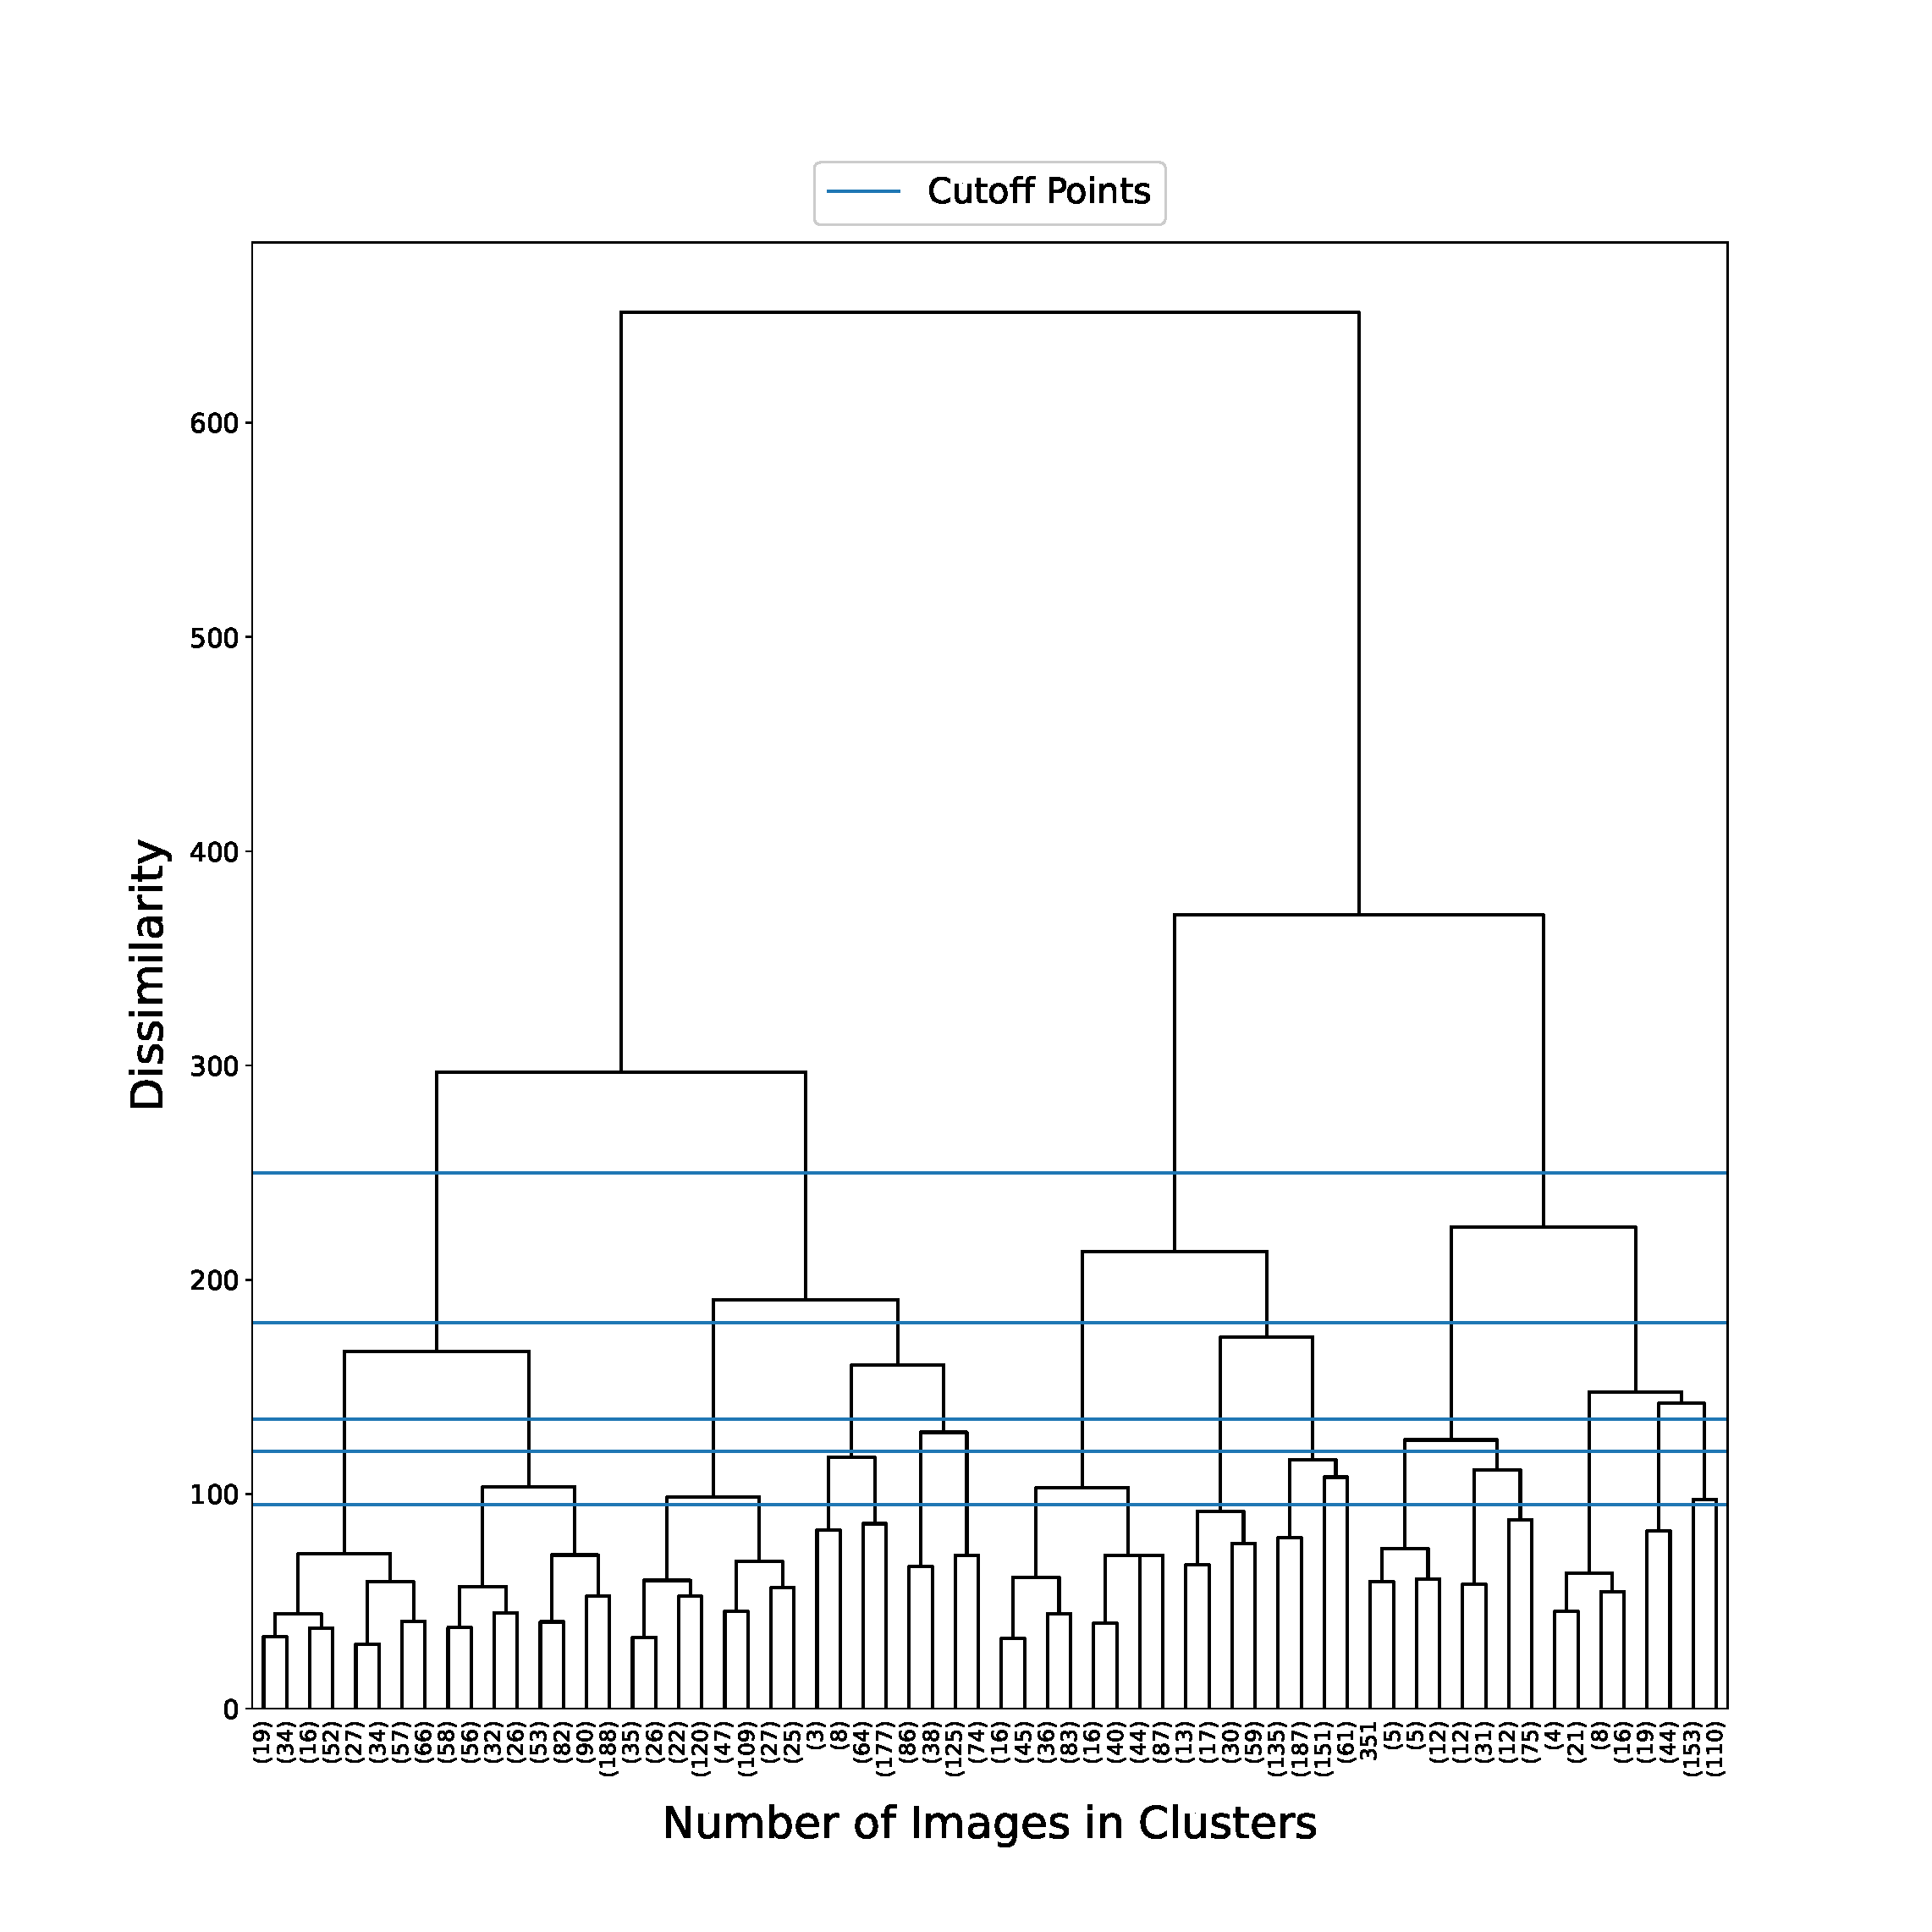
\includegraphics[width=1\textwidth]{Images/hierarcial_clustering_dendrogram.eps}
        %     \caption{Schematic diagram representing the tree-like structure of hierarchical clustering where the vertical lines represent the various clusters and the horizontal lines represent the points at which these clusters come together. The horizontal blue lines represent various cutoff points, splitting our galaxy images into 4, 7, 12, 14 and 22 groups. The y-axis represents the dissimilarity of the images within each cluster.}
        %     \label{Dendrogram}
        % \end{figure}
        
        % In Figure \ref{Dendrogram}, we can see how hierarchical clustering is working for our images. Because we have so many in our dataset, I have cut this diagram off to show 6 layers, showing 64 clusters. The numbers across the x-axis represent the number of images in each of those 64 clusters. The y-axis represents the dissimilarity of the images, the lower the value, the closer in our 32-dimensional space, and therefore more similar the images within that cluster are. 
        
        % By looking at the dendrogram, we can choose various cutoff points, represented by the horizontal, blue lines, to help to choose how many clusters we want. It is best to pick cutoff points where there is a good level of separation in dissimilarity between clusters above and below the point. For example, in Figure \ref{Dendrogram}, I have shown some cutoff points with dissimilarity levels of 250, 180, 135, 120 and 95 resulting in 4, 7, 12, 14 and 22 clusters respectively. Any cutoff point can be chosen, and we can go up to as many clusters as we would like.
    

\newpage

\section{Results} 
\label{Results}

    \subsection{Optimal Number of Extracted Features}
    \label{no_extracted_features}

    A well-trained model which has found meaningful patterns in the images will be able to accurately reconstruct galaxy images. Additionally, a well-trained model implies that the extracted features provide an accurate encoding of the original images. 
    
    To find the optimal number of extracted features, we must strike a balance between extracting enough features to produce accurate reconstructions while ensuring that they are astronomically and scientifically meaningful.

%    \begin{figure}[H]
%        \centering
%        \begin{subfigure}[b]{0.48\textwidth}
%            \centering
%            \includegraphics[width=\textwidth]{Images/rand_extracted_feat_vs_loss.eps}
%            \caption{}
%            \label{extracted_feature_loss}
%        \end{subfigure}
%        % \hfill
%        \begin{subfigure}[b]{0.48\textwidth}
%            \centering
%            \includegraphics[width=\textwidth]{Images/rand_meaningful_extracted_features_0-3_abs.eps}
%            \caption{}
%            \label{meaningful_extracted_features}
%        \end{subfigure}
%        \caption{\ref{extracted_feature_loss} shows the loss of reconstructions (root-mean-squared loss between the original images and their reconstructions) against the number of extracted features. This is plotted for both the training data and validation data (a subset of the dataaset (200 images) not used to train the model). \ref{meaningful_extracted_features} shows the number of meaningful extracted features against the total number of extracted features. I have defined a meaningful extracted feature as a feature with a correlation coefficient $\rho \geq 0.2$ with at least one of the galaxy properties discussed in sections \ref{structual_measurements} and \ref{physical_propeties}). Error bars are obtained by training the model 3 times for each extracted feature. The points represent the median value of the 3 runs.}
%        \label{optimal_exracted_features}
%    \end{figure}


    % \begin{figure}[H]
    %     \centering
    %     \includegraphics[width=\textwidth]{Images/rand_extracted_feat_vs_loss.eps}
    %     \caption{loss of reconstructions (root-mean-squared loss between the original images and their reconstructions) against the number of extracted features. This is plotted for both the training data and validation data (a subset of the dataaset (200 images) not used to train the model). Error bars are obtained by training the model 3 times for each extracted feature. The points represent the median value of the 3 runs.}
    %     \label{extracted_feature_loss}
    % \end{figure}

    % \begin{figure}[H]
    %     \centering
    %     \includegraphics[width=\textwidth]{Images/rand_meaningful_extracted_features.eps}
    %     \caption{the number of meaningful extracted features against the total number of extracted features. I have defined a meaningful extracted feature as a feature with a correlation coefficient $\rho \geq 0.2$ with at least one of the galaxy properties discussed in sections \ref{structual_measurements} and \ref{physical_propeties}). Error bars are obtained by training the model 3 times for each extracted feature. The points represent the median value of the 3 runs.}
    %     \label{meaningful_extracted_features}
    % \end{figure}
    
    
    Figure \ref{extracted_feature_loss} shows that the more extracted features we have, the more accurate our model is. This is expected as more extracted features means the decoder has more information about each image so should be able to form more accurate reconstructions. However, the rate at which accuracy increases with extracted features, starts to decrease at higher numbers.

    Figure \ref{meaningful_extracted_features} shows that as more features are extracted, the number of meaningful extracted features (an extracted feature with a correlation coefficient $\rho \geq 0.2$ with at least one of the galaxy properties discussed in sections \ref{structual_measurements} and \ref{physical_propeties}) increases as the model extracts more features. However, again, the rate of extracting meaningful features starts to decrease for higher numbers of extracted features showing that we aren't actually getting any more astronomical or scientific information out of the images, meaning some of the extracted features start to become meaningless. Given the galaxies will be categorised by their extracted features (see section \ref{Clustering Results}) and we want the model to categorise the galaxies based on their morphology, we have to ensure that the majority of the extracted features are scientifically meaningful.

    To strike a balance between these two considerations, I have chosen to configure the model to extract ************************ features.


    \subsection{Representation of the Machine Features}
    \label{Representation of the Machine Features}

    
        \subsubsection{Comparison with Structural Measurements}
        \label{structual_measurements}

        Structural measurements represent the observable characteristics and appearance of galaxies \cite{structure_measurement}. One key structure measurement is the Sersic Index \cite{sersic_index}. The Sersic index is a scale representing the light profile of a galaxy. The more the light is centrally concentrated, the higher the Sersic index and the more spread out the light profile is, the lower the Sersic index. This means bulge-dominated galaxies, such as ellipticals typically have higher Sersic indices than disk structures such as spiral galaxies.
        
        The EAGLE database \cite{eagle_catalogue_public_release} provides 3 images for each galaxy in each simulation. This includes a face-on perspective, an edge-on perspective and a random orientation. To better match real observational data, I have chosen to sample the images with random orientations. This introduces another key structure measurement - the position angle. The position angle is the angle between the line of sight and the plane of the galaxy. Position angles close to 0$^{\circ}$ represent face-on images, and values closer to 90$^{\circ}$ (or -90$^{\circ}$) represent edge-on images.

        Another key structural measurement is the axis ratio. This is the ratio between the semi-major and semi-minor axes and is a measure of how elongated the galaxy is.


        \begin{figure}[H]
            \centering
            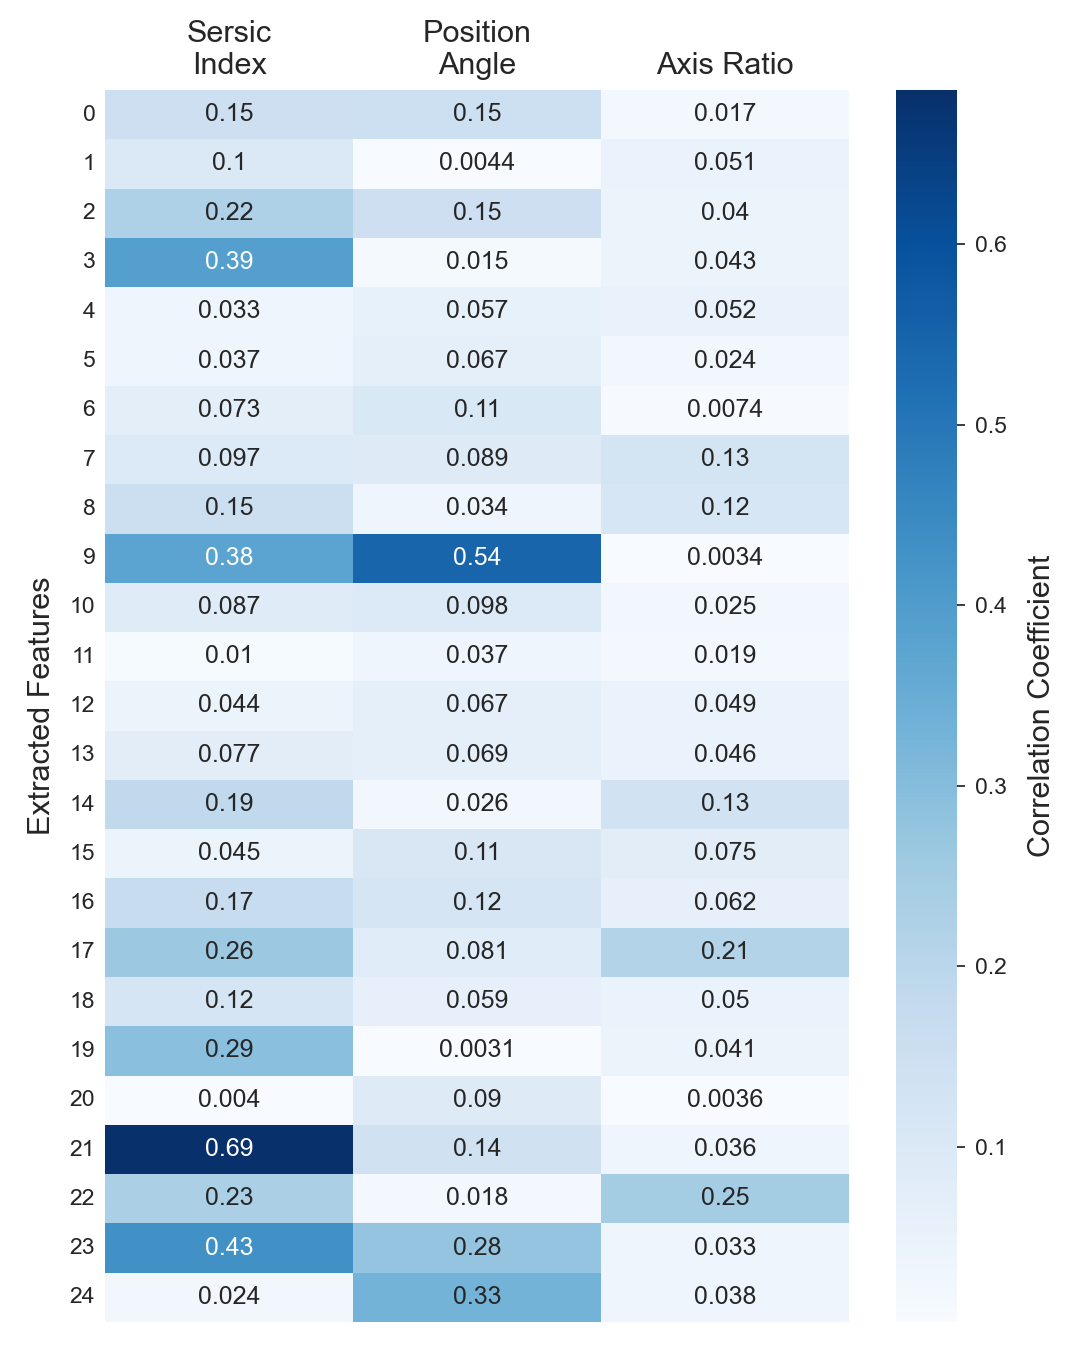
\includegraphics[width=0.8\textwidth]{Images/25_feature_structure_property_correlation_2.png}
            \caption{Correlation coefficient, $\rho$ between each of the 25 extracted features and the Sersic index, position angle and axis ratio. Structural measurements were obtained from the EAGLE database \cite{eagle_catalogue_public_release}. The numbers corresponding to each extracted feature have no scientific meaning, they are simply used to identify each feature.}
            \label{structure_correlation}
        \end{figure}

        
        Structure measurements can be obtained directly from images so we would expect to see some correlation between the extracted features and the Sersic index, position angle and axis ratio.

        ***************

        


        

        \subsubsection{Comparison with Physical Properties}
        \label{physical_propeties}

        Physical galaxy properties relate to more intrinsic quantities, and therefore can't be directly obtained from images. For example, the star formation rate is the mass of stars formed per unit time \cite{sfr_definition}. However, there is some correlation between the extracted features and some physical properties.

        We compare the extracted features to the following galaxy properties, semi-major axis, star formation rate, *************************************** from the EAGLE database \cite{eagle_catalogue_public_release}.

        \begin{figure}[H]
            \centering
            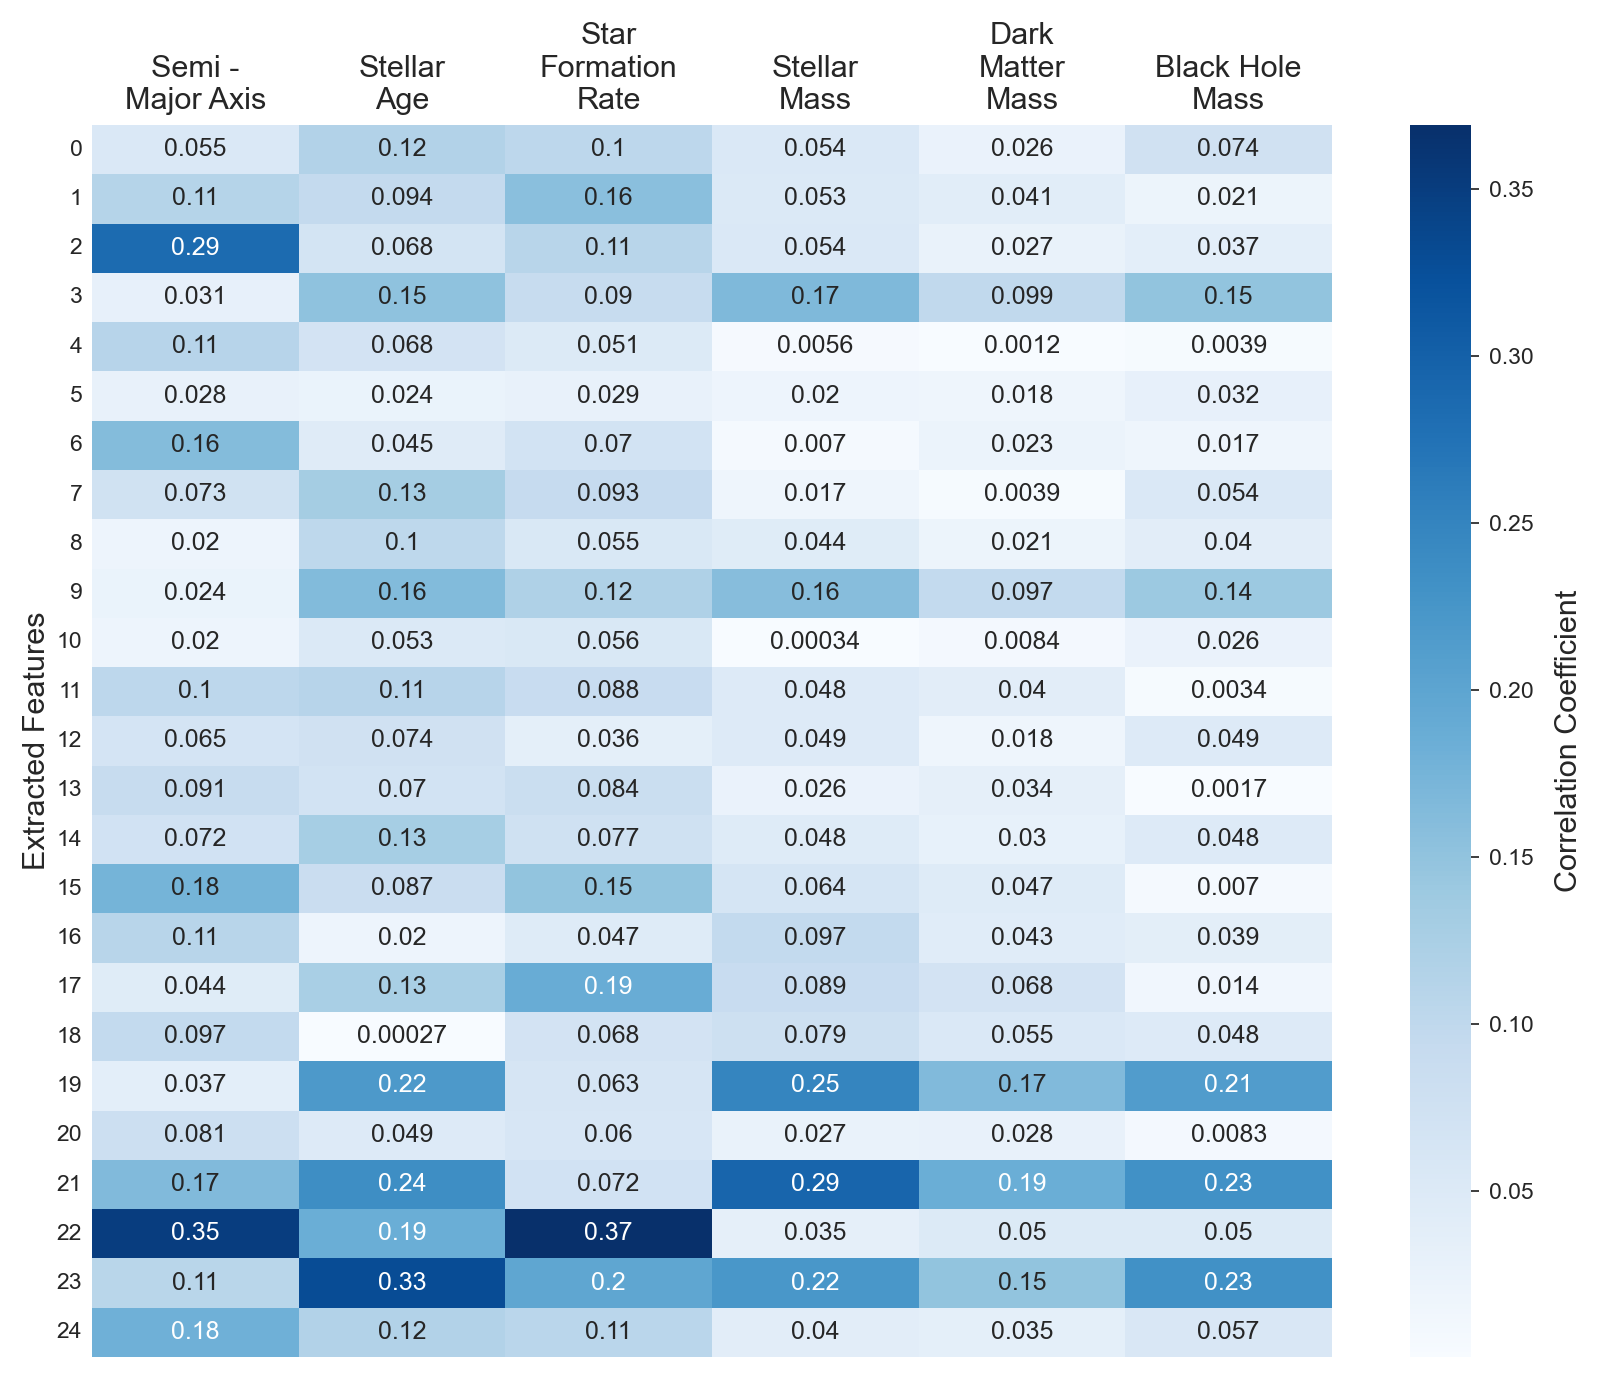
\includegraphics[width=\textwidth]{Images/25_feature_physical_property_correlation_2.png}
            \caption{Correlation coefficient, $\rho$ between each of the 25 extracted features and the semi-major axis, stellar age, star formation rate, stellar mass, dark matter mass and black hole mass.}
            \label{physical_correlation}
        \end{figure}

        Although these physical properties can't normally be obtained directly from the images, we can actually see some correlation ......................

        



        \subsubsection{Comparison with Visual Inspection}
        \label{visual_inspection}

        By holding all extracted features constant (at the median values for all galaxy images) apart from one, we can use the decoder to form reconstructions to get a visual representation of each of the extracted features.

%        \begin{figure}[H]
%            \centering
%            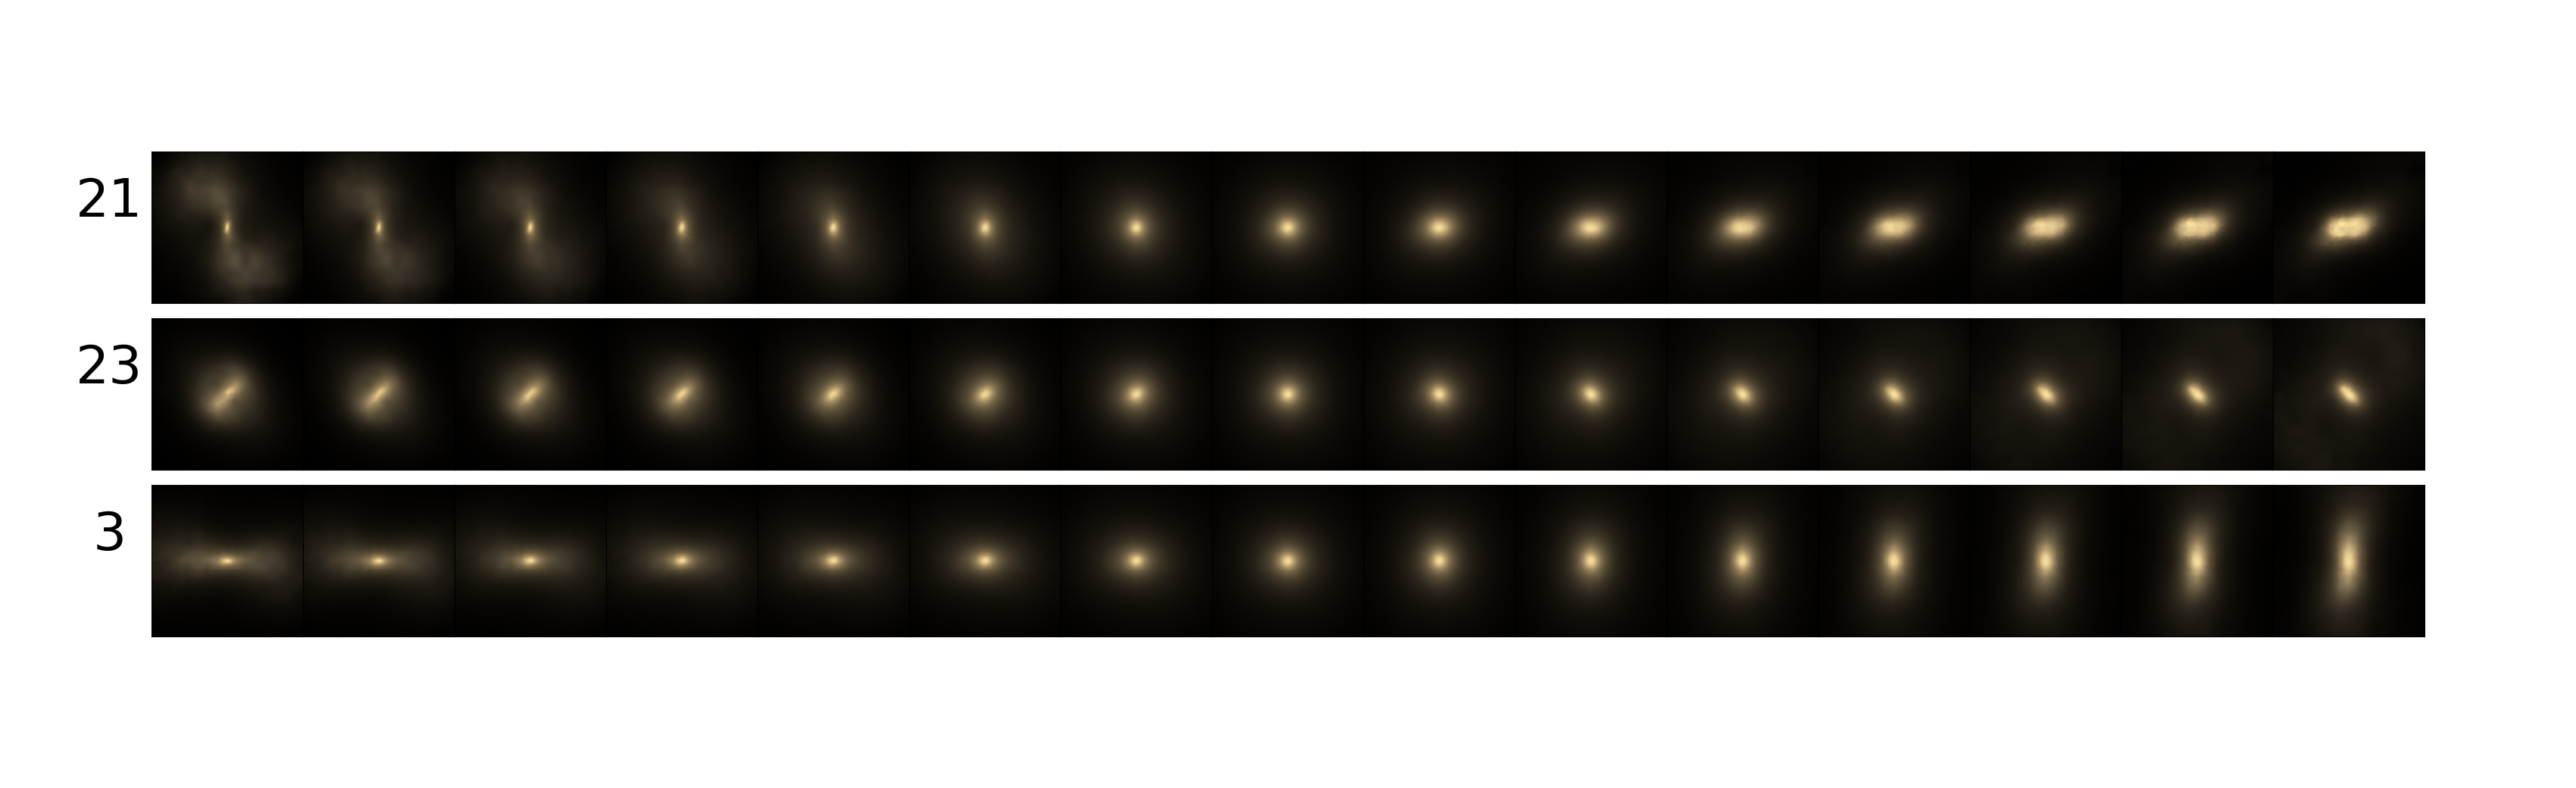
\includegraphics[width=\textwidth]{Images/latent_25_features_2_sersic.eps}
%            \caption{Reconstructions by varying features 21, 23 and 3 individually while holding all others constant}
%            \label{sersic_reconstructions}
%        \end{figure}

        \vspace{5mm}

        **********************
        Position Angle and other rotation Features
        **********************

        \vspace{5mm}

        \vspace{5mm}

        **********************
        Other physical properties eg. sfr???
        **********************

        \vspace{5mm}

        \vspace{5mm}

        **********************
        No change features (with correlation), machine looking further
        **********************

        \vspace{5mm}
        

        Talk about position angle and rotation angle making it more difficult. Not much we can do about rotation angle (we can't rotate images) but for position angle, we can remove these features from the clustering algorithm
        


    \subsection{Catagorisation of Galaxies}

        \subsubsection{Clustering Results}
        \label{Clustering Results}

        Number of clusters, dendrogram?. Emmiting certain features for position angle. Why we can't remove the effect of other rotations.
        
        \subsubsection{Comparison with Structural Measurements}
        \label{Structual Clusters}


        
        \subsubsection{Copmarison with Physical Properties}
        \label{Physical Clusters}

        
        % \subsubsection{*** Comparison with Visual Morphology ***}

        % *** May not have time to include ***

    








    % \subsection{Galaxy Property Extraction}
    % \label{Propety Extraction}
    
    %     We have chosen to extract 32 features for each galaxy (as explained in part \ref{Feature Extraction}) which gives us 32 numerical values for each image. We want to know if any of these extracted features are related to any galaxy properties. From the EAGLE Database \cite{trayford}, we can access many galaxy properties. Additionally, we can use the supplementary file given by Anna de Graaff \cite{de_Graaff_mass_size_relation} to find some galaxy properties for a subset of the RefL0100N1504 \cite{trayford} dataset.
        
    %     \begin{figure}[H]
    %         \centering
    %         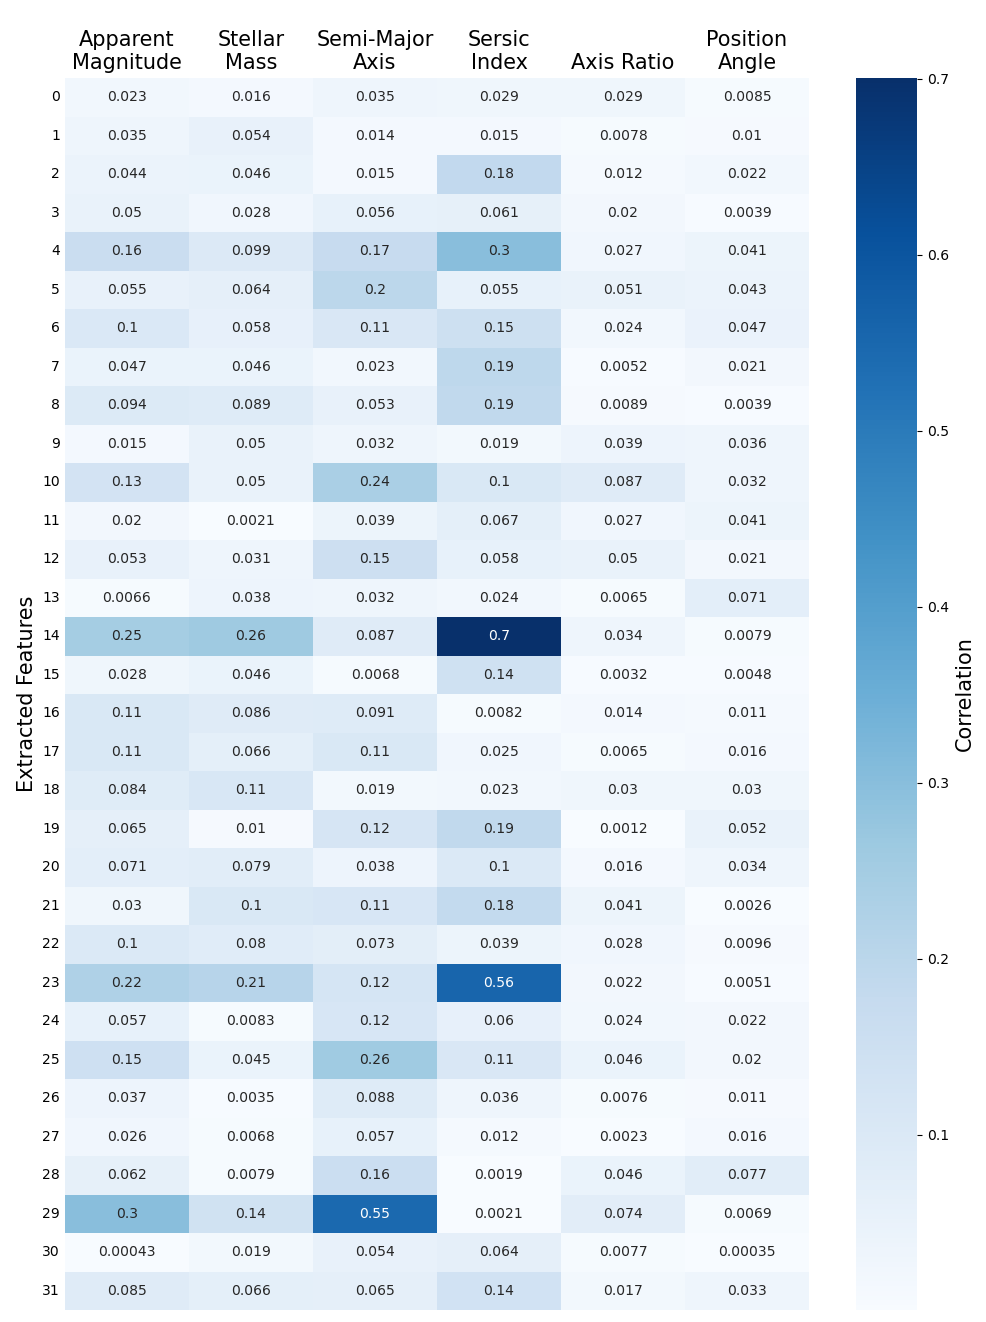
\includegraphics[width=0.6\textwidth]{Images/32_feature_property_correlation.png}
    %         \caption{Correlation coefficient of each extracted feature with each galaxy property from the supplemental file from \cite{de_Graaff_mass_size_relation}}
    %         \label{Supp Property Correlation}
    %     \end{figure}
        
    %     In Figure \ref{Supp Property Correlation} we show the correlation coefficient between each extracted feature and each galaxy property. The darker points represent a strong correlation and we can see that there is a very obvious correlation between feature 14 and the Sersic Index of the galaxy (feature 23 also seems to be quite strongly correlated to the Sersic Index).
        
    %     There is a small amount of correlation between feature 29 and the Apparent Magnitude of our galaxies. However, we have a much stronger correlation between this feature and the Semi-Major axis. This means that the resizing algorithm described in Section \ref{Image Resizing} is working well to remove the effect of the model focussing on the apparent size of our galaxy, and instead is picking out physical galaxy properties. If we remove the resizing algorithm, we obtain a correlation coefficient of 0.51 between a feature and the apparent magnitude which is significantly higher than that shown in Figure \ref{Supp Property Correlation}. Additionally, without the resizing algorithm, we also only get a correlation coefficient of 0.6 between a feature and the Sersic index which is much lower than 0.7, as shown in Figure \ref{Supp Property Correlation}. This further proves that the resizing algorithm is working well to highlight physical galaxy properties rather than arbitrary image properties.
        
    %     \vspace{10mm}
    %     \noindent *** Compare with evolutionary history properties eg. merger rate, numbers of mergers experienced, star formation rate, abundance of heavy elements, active galaxy nuclei activity
        
    %     \vspace{10mm}
        
    %     \noindent *** Compare with other properties eg. dark halo mass, blackhole mass, gas mass
    %     \vspace{10mm}
        
    
    
    % \subsection{Categorising Galaxies}
    % \label{Categorising Galaxies}
    
    %     \begin{figure}[H]
    %         \centering
    %         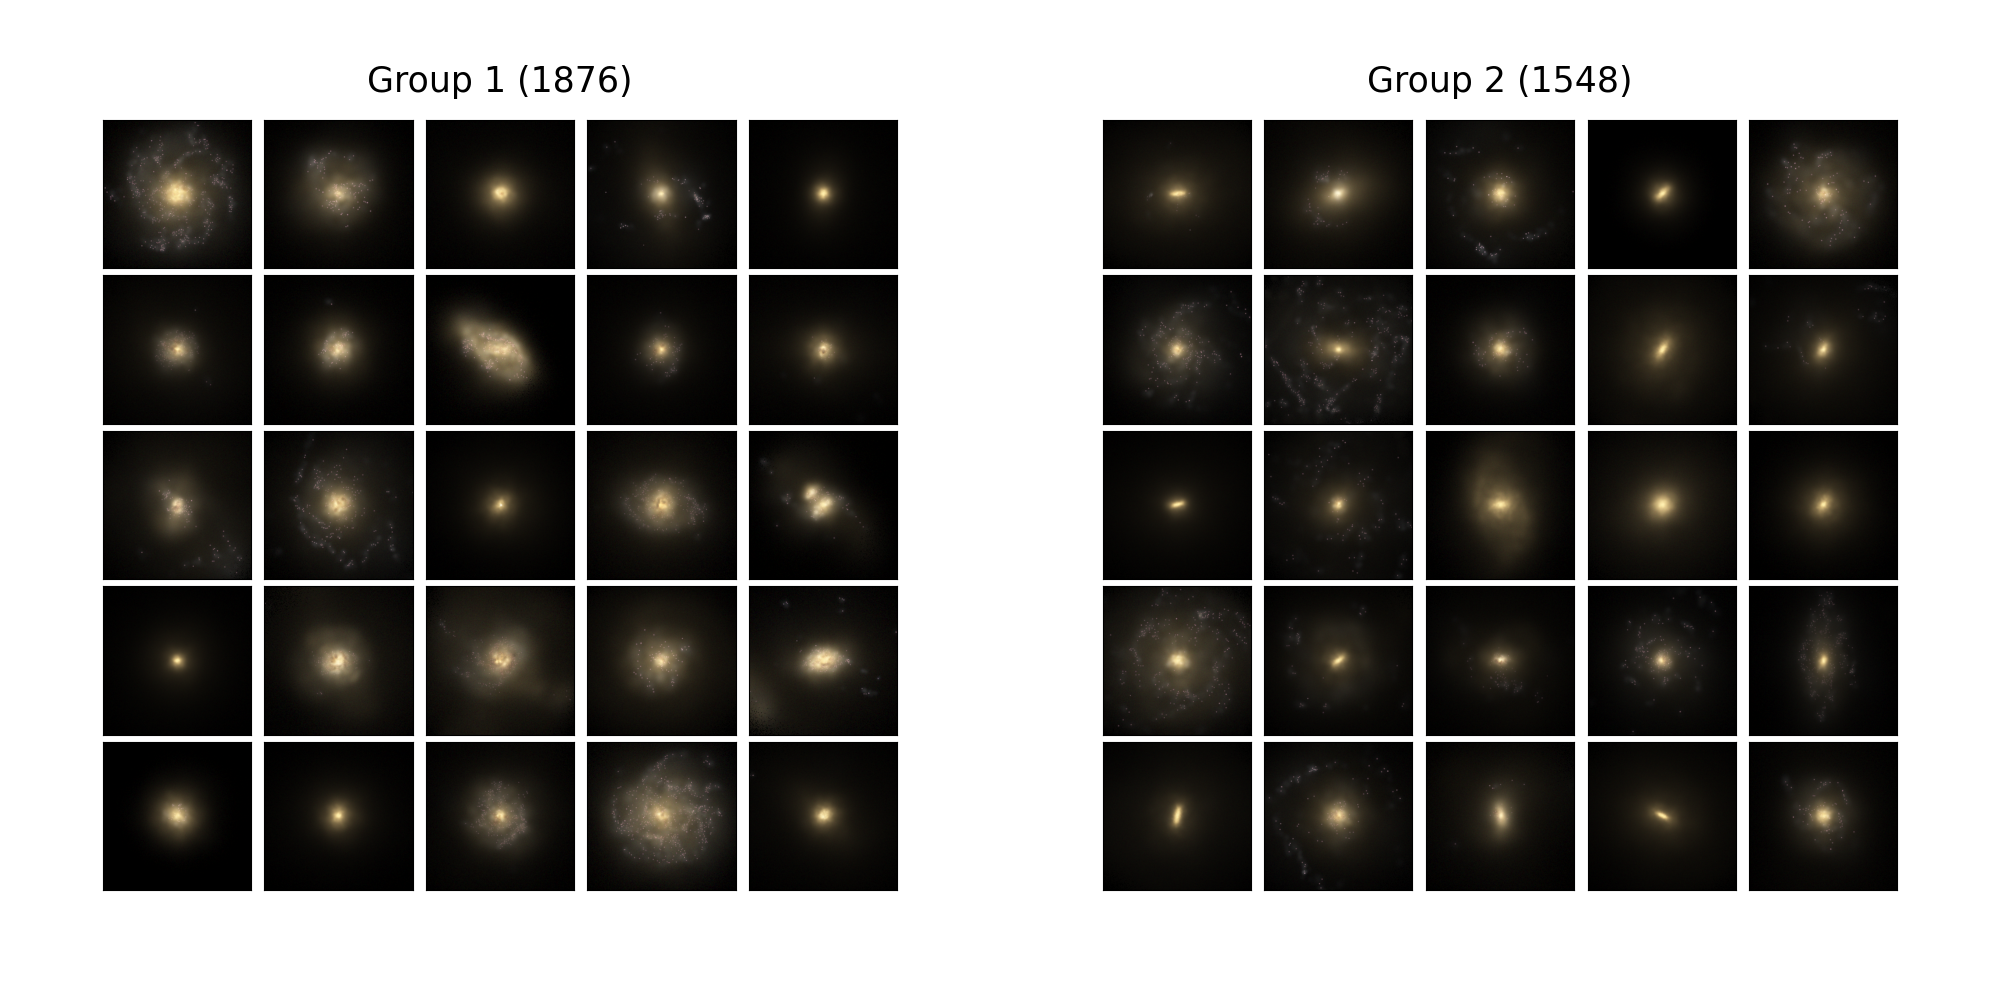
\includegraphics[width=0.75\textwidth]{Images/2_cluster_32_feature_originals_25.png}
    %         \caption{RefL0100N1504 images \cite{trayford} grouped into 2 clusters}
    %         \label{2 Groups}
    %     \end{figure}
        
    %     From our clustering algorithm described in Section \ref{Clustering}, we can look at what images are being grouped into each cluster. If we start with 2 clusters, shown in Figure \ref{2 Groups}, for example, we can see that our galaxies appear to be split into a more featured group (Group 1) and a less featured group (Group 2). Galaxies in Group 2 appear to be more elliptical in shape, while galaxies in Group 1 appear to be more spiral-like.
        
    %     \vspace{10mm}
    %     \noindent  *** Figures of images split into 4 and 7 groups, explain how the groups are formed (from the clustering algorithm). For example, for 4 groups, the original group 1 splits into two groups, group 1-1 and group 1-2, explain the differences between groups 1-1 and 1-2 and how they came from group 1.
    %     \vspace{10mm}
    
    
    
    % \subsection{Catagorised Galaxy Properties}
    
    %     In part \ref{Propety Extraction}, we have found some correlation between certain extracted features and galaxy properties and in part \ref{Categorising Galaxies}, we have grouped similar galaxies together into clusters. We can now bring that together and look at how each cluster compares to our galaxy properties.
        
    %     \begin{figure}[H]
    %         \centering
    %         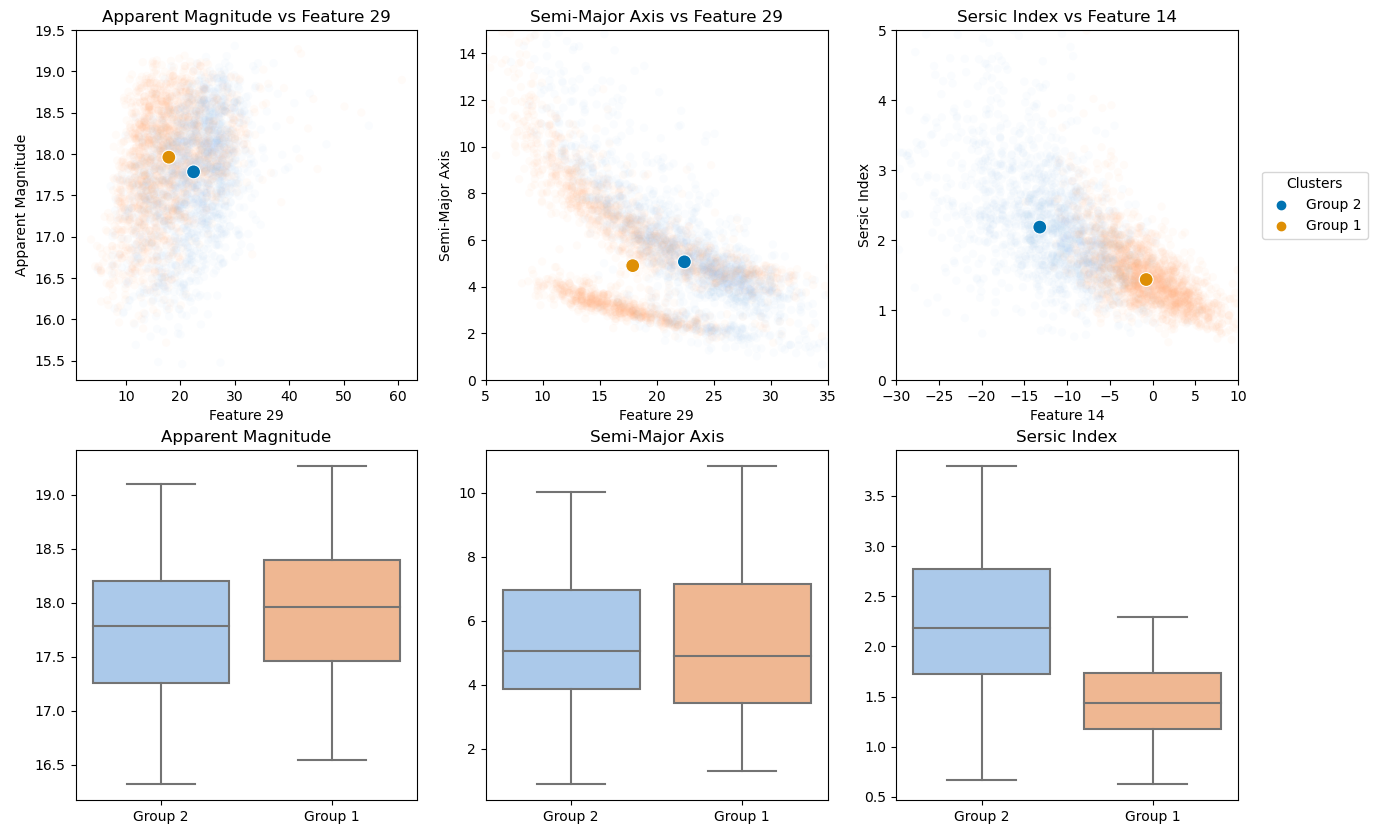
\includegraphics[width=0.7\textwidth]{Images/2_cluster_properties.png}
    %         \caption{2 Clustered Correlation between strongly correlated extracted features and galaxy properties}
    %         \label{2 Cluster Properties}
    %     \end{figure}
        
    %     Explain what the above figure shows. Also, show the correlation between extracted features and galaxy properties with a higher number of clusters (I wouldn't include the box plots for this, it would be more to show the trend and how the clusters are distributed.
        
    %     Plot properties against each other, showing how they are correlated with each other and how the different clusters are distributed along this correlation
    
    
\newpage

\section{Conclusions}
\label{Conclusions}

\section{Summary for a General Audience}
\label{General Audience Summary}


\vspace{5mm}
***** Does this go before or after references? *****
\vspace{5mm}



\section{Future Work}
\label{Future Work}

Why I chose redshift 0.1 - calibrated at low redshift 

(https://academic.oup.com/mnras/article/450/2/1937/984366#17138259)

Higher resolution images, much more control over rotations (align semi major axis) and cropping (same apparent size)

\vspace{5mm}
******* DOI In References *******
\vspace{5mm}

% Can be used with other simulations (eg. Illustris) and with real images. Can also be used to compare simulations to see what is missing between them

% \begin{acknowledgments}

% (OPTIONAL) The author would like to thank...

% \end{acknowledgments}

\newpage

\printbibliography


\end{document}